%% !TeX program = pdflatex
\documentclass[presentatie.tex]{subfiles}

\csname inputexit\endcsname
\csname inputentrance\endcsname
\def\named#1{}

\begin{document}
    \clearrecentlist

    \inputentrance\named{mytest}
    \begin{frame}
        \frametitle{\LaTeX{} vs Word}

        \begin{columns}
            \begin{column}{0.5\textwidth}
                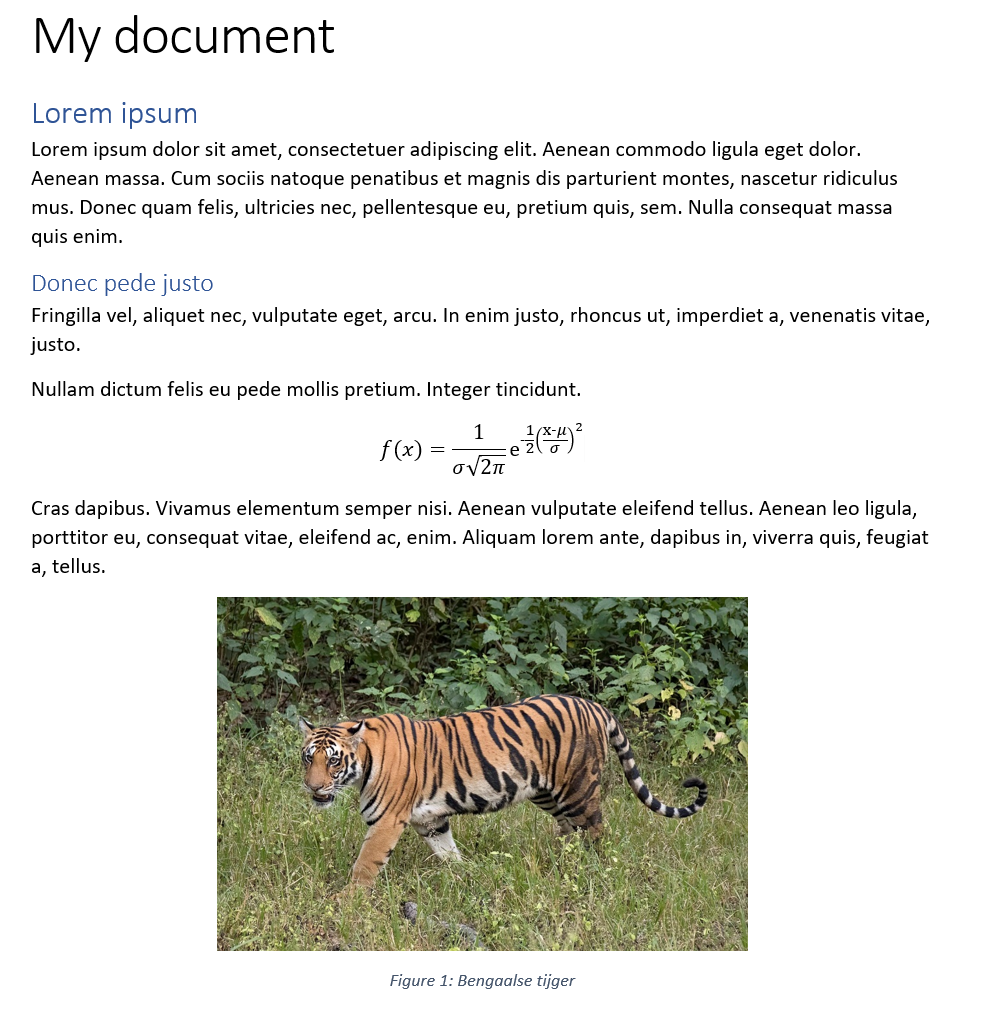
\includegraphics[width=\linewidth,height=0.8\textheight,keepaspectratio]{assets/basicDocWordSnippet.png}
            \end{column}
            \begin{column}{0.5\textwidth}
                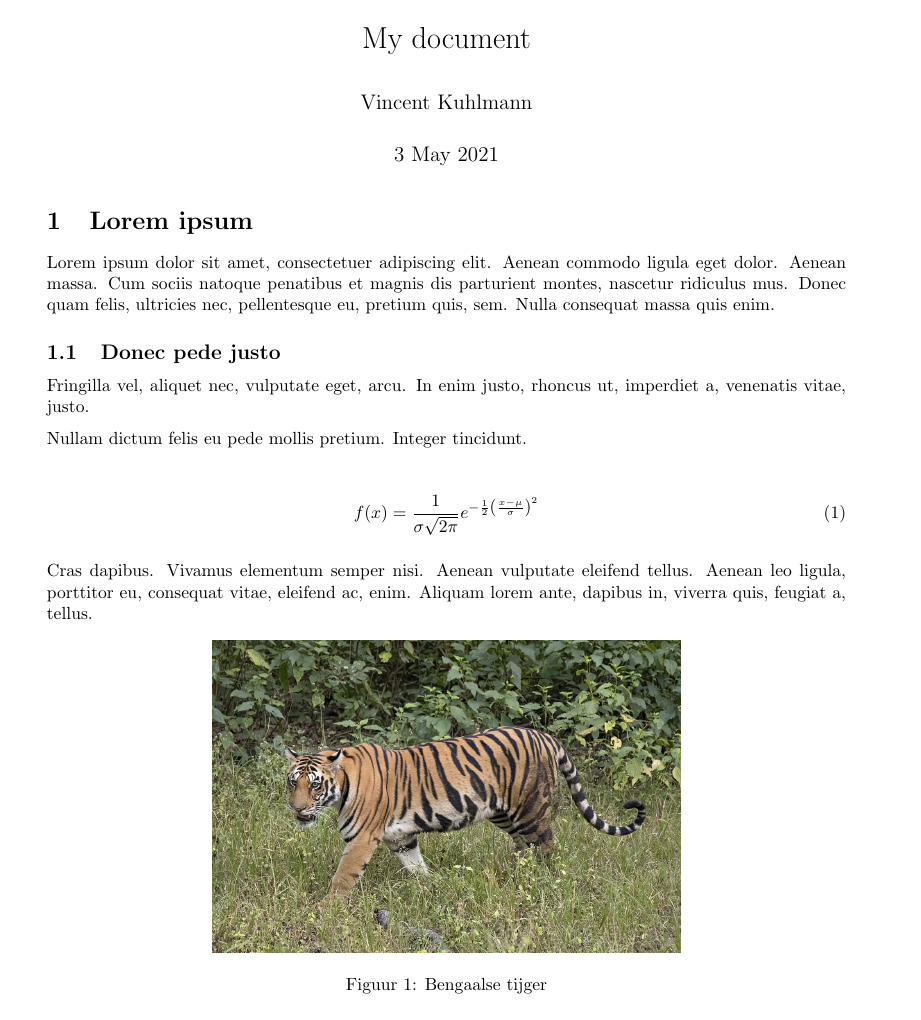
\includegraphics[width=\linewidth,height=0.8\textheight,keepaspectratio]{assets/basicDocLaTeXSnippet.png}
            \end{column}
        \end{columns}
    \end{frame}
    \inputexit

    \begin{frame}
        \frametitle{\LaTeX{} vs Word}

        \bgroup
        \setlength{\fboxsep}{0pt}
        \fbox{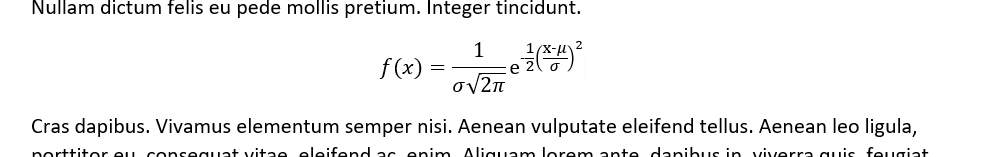
\includegraphics[width=\linewidth,height=0.5\textheight,keepaspectratio]{assets/basicDocWordSnippetEq.png}}
        \medskip

        \fbox{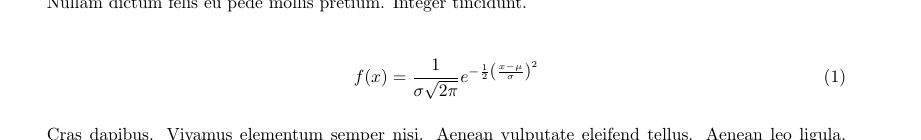
\includegraphics[width=\linewidth,height=0.5\textheight,keepaspectratio]{assets/basicDocLaTeXSnippetEq.png}}
        \egroup
    \end{frame}

    \inputentrance\named{motorkap}
    \begin{saveblock}{basicDocCode}
        \begin{highlightblock}[linewidth=\textwidth,gobble=12]
            \title{My document}
            \author{Vincent Kuhlmann}
            \date{3 May 2021}

            \begin{document}
            \maketitle
            \section{Lorem ipsum}
            Lorem ipsum dolor sit amet, consectetuer ...

            \begin{align}
                f(x) = \dfrac{1}{\sigma\sqrt{2\pi}} e^{
                        -\frac{1}{2}\left(\frac{x-\mu}{\sigma}\right)^2}
            \end{align}
        \end{highlightblock}
    \end{saveblock}

    \begin{frame}
        \frametitle{\LaTeX{} vs Word}

        Onder de motorkap: groot verschil.

        Word: Visueel, \LaTeX: Code (tekst).

        \pause
        \medskip

        \begin{columns}[t]%
            \begin{column}{0.6\textwidth}
                \adjustbox{max height=0.6\textheight}{
                    \useblock{basicDocCode}
                }
            \end{column}%
            \begin{column}{0.4\textwidth}%
                \adjustbox{fbox=0.5pt 0pt 0pt,margin=-30pt 0pt 0pt 0pt,set height=0pt}{%
                    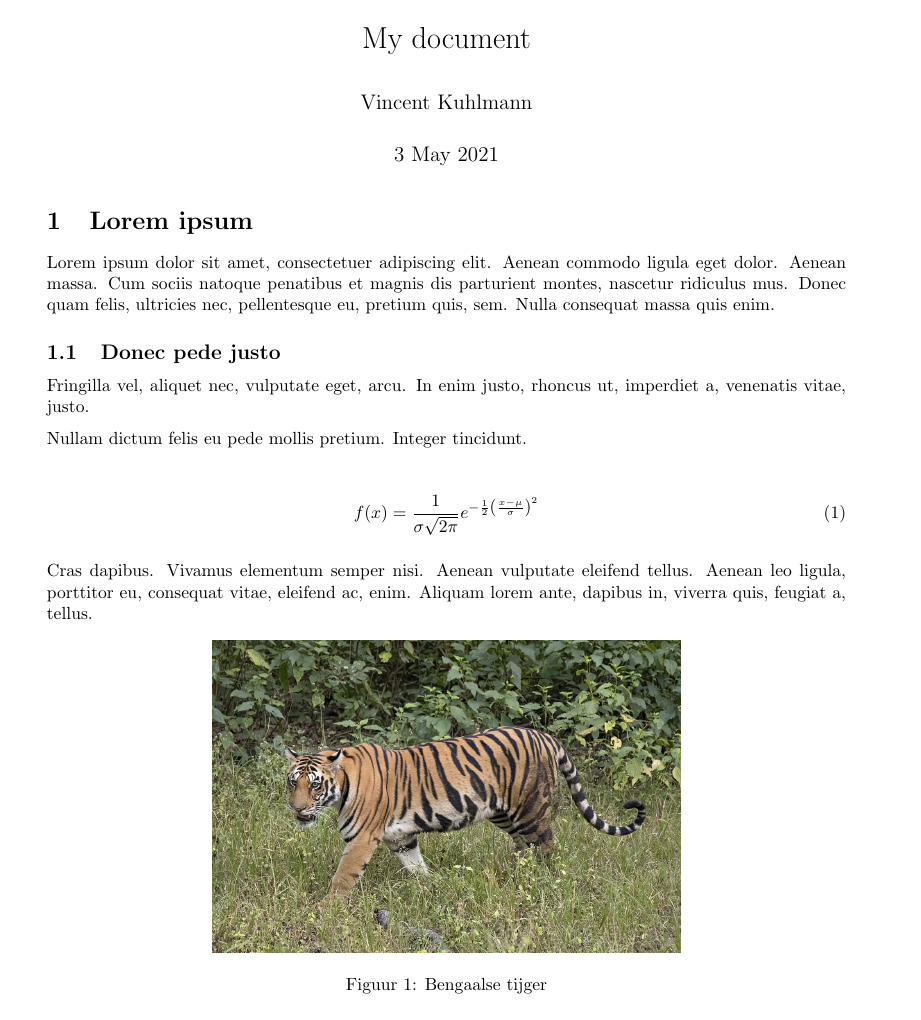
\includegraphics[width=1.6\linewidth,height=0.9\textheight,keepaspectratio]{assets/basicDocLaTeXSnippet.png}%
                }
            \end{column}%
        \end{columns}
    \end{frame}
    \inputexit

    \begin{frame}<1-4>[label=codeoverview]
        \frametitle{Code vs Visueel}

        \parbox[c][0.8\textheight]{0.35\textwidth}{
            \begin{itemize}
                \item<1-> Websites \& Apps
                \par\uncover<3->{\textbf{Complex}}

                \item<4-> Wikipedia
                \par\uncover<5->{\textbf{Consistent}}

                \item<6-> WhatsApp
                \par\uncover<7->{\textbf{Uitbreidbaar}}
            \end{itemize}
        }\hfil
        %\parbox[c]{1pt}{\textcolor{red}{\rule{0.5pt}{0.3\textheight}}}%
        \hfil
        \parbox[c]{0.6\textwidth}{
        \unless\ifishandout
            \only<1>{
                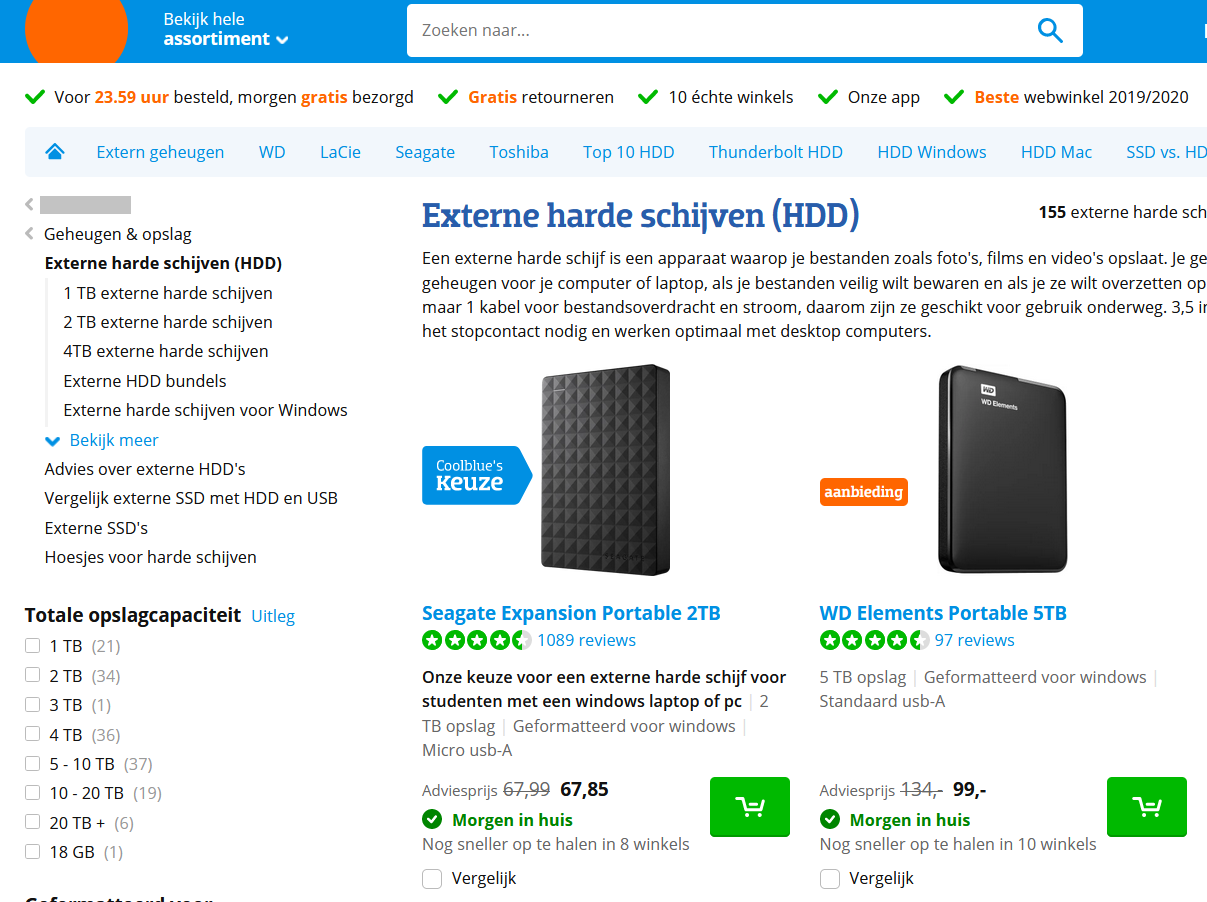
\includegraphics[
                    width=\linewidth,height=0.8\textheight,keepaspectratio
                ]{assets/websiteVisual.png}
            }
            \only<2-3>{
            \adjustbox{
            trim=0pt {0.5\height} {0.5\width} 0pt,clip,width=\linewidth
            }{%
            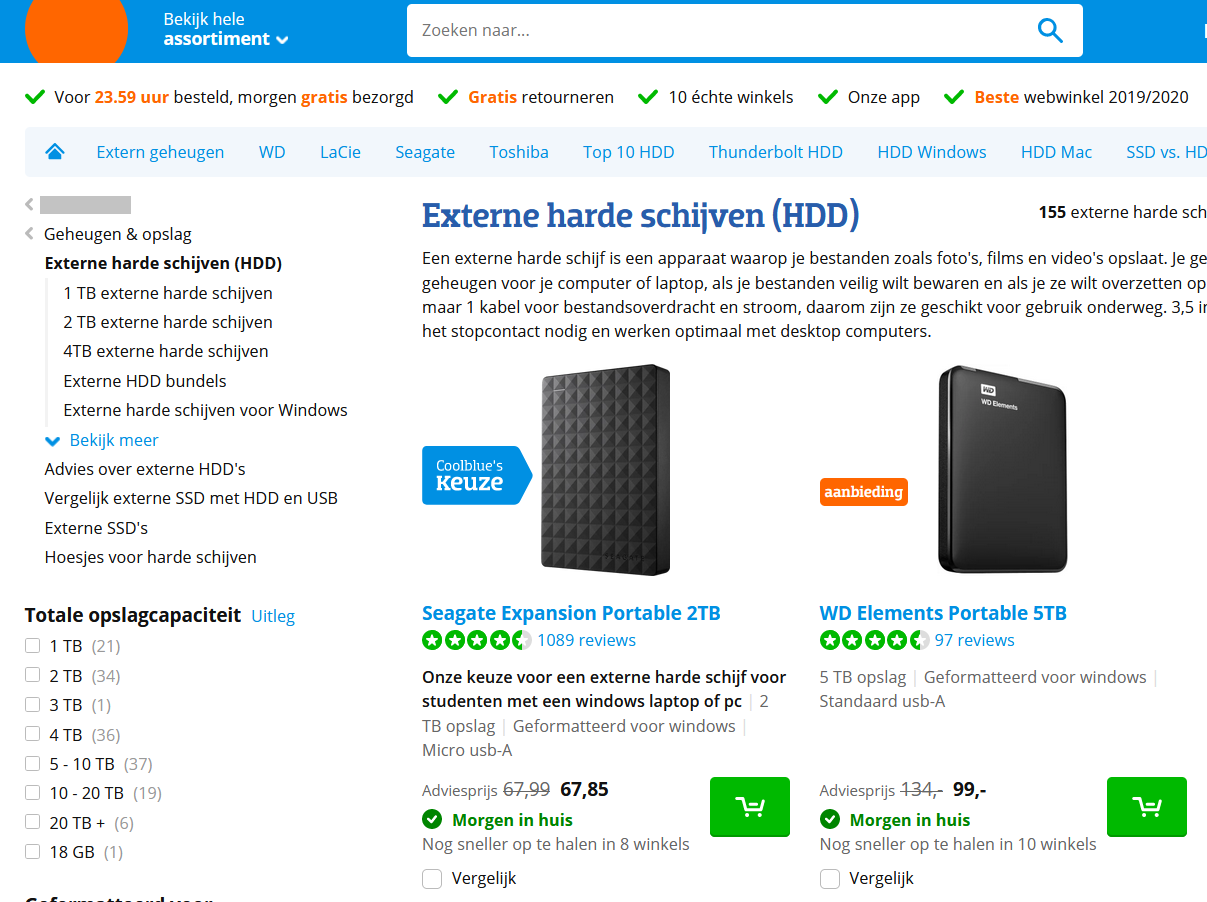
\includegraphics[
                width=\linewidth,height=0.8\textheight,keepaspectratio
            ]{assets/websiteVisual.png}%
            }
            }
            \only<4-5>{
                \centering
                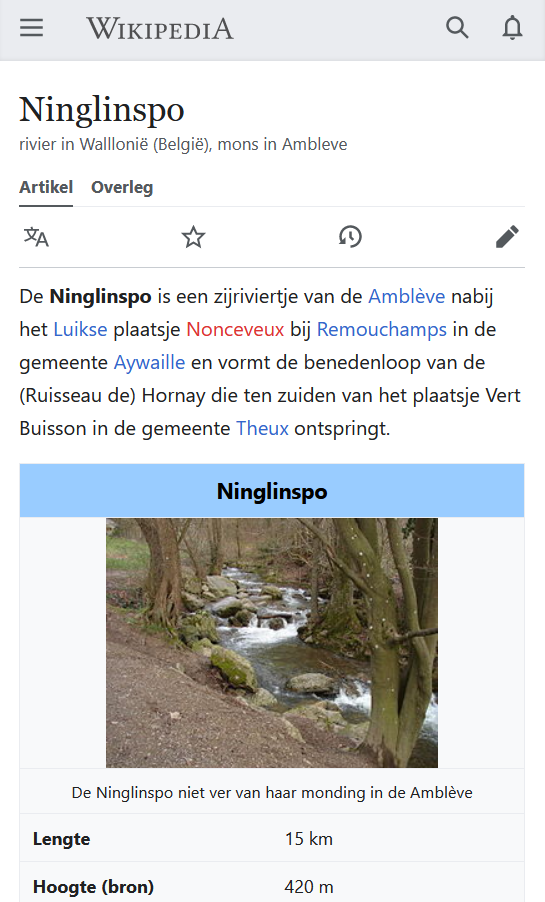
\includegraphics[width=\linewidth,height=0.8\textheight,keepaspectratio]{assets/wikipediaVisual}
                %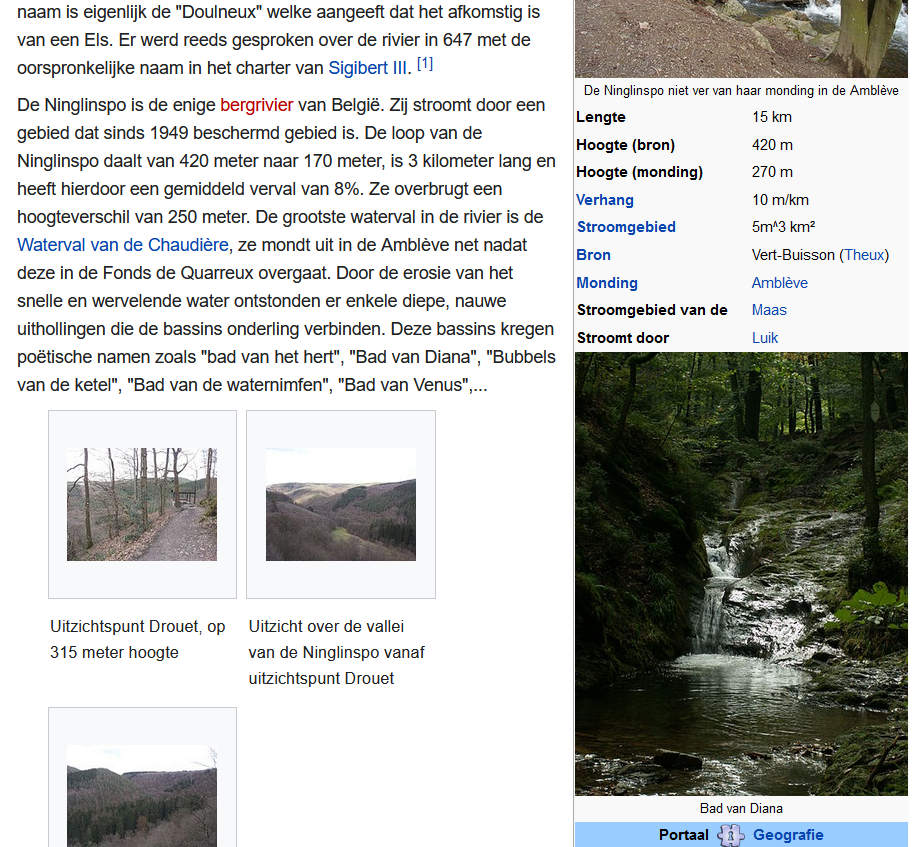
\includegraphics[width=\linewidth,height=0.8\textheight,keepaspectratio]{assets/wikipediaVisual2}
            }
        \fi
        \only<6-7>{
            
\includegraphics[width=\linewidth]{assets/whatsappStyles2.png}

            \bigskip

            %
\includegraphics[width=\linewidth]{whatsappStylesResultCropped.jpg}
            
\includegraphics[width=\linewidth]{assets/whatsappStylesResult2.png}
        }
        }
    \end{frame}

    \begin{saveblock}{ninglinspoFragment1}
        \begin{Verbatim}[tabsize=4,gobble=8]
            {{Infobox rivier
            | naam          = Ninglinspo
            | afbeelding    = Ninglinspo - arrivée d
            | onderschrift  = De Ninglinspo niet ver
            | lengte        = 15
            | hoogte        = 420
            | hoogtemonding = 270
            | verhang       =
            | debiet        =
        \end{Verbatim}
    \end{saveblock}

    \begin{saveblock}{ninglinspoFragment2}
        \begin{Verbatim}[tabsize=4,gobble=8]
            De oorspronkelijke naam is eigenlijk de "Doulneu
            een Els. Er werd reeds gesproken over de rivier
            charter van [[Sigibert III]].
            <ref>informatiebord aan de monding van de Ningli
        \end{Verbatim}
    \end{saveblock}

    \begin{frame}
        \frametitle{Code vs Visueel}

        % \begin{columns}
        %    \begin{column}{0.45\textwidth}
        %\centering
        \adjustbox{
            trim=0pt 0pt 5em 0pt,
            max height=0.9\textheight,max width=0.5\linewidth,
            %fbox=1pt 0pt 2pt,
            cframe=green!50!white 0.5pt 0pt 2pt,
            valign=M
        }{
            \useblock{ninglinspoFragment1}
        }%
        %\hspace{2pt}%
        \adjustbox{
            cframe=blue!50!white 0.5pt 0pt 0pt,
            valign=M
        }{%
            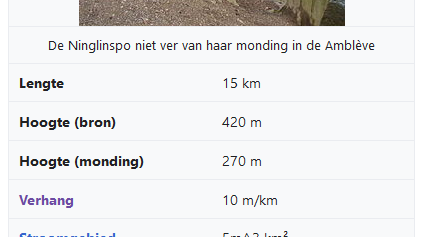
\includegraphics[
                trim=7pt 0pt 7pt 0pt,clip,
                height=0.5\textheight,width=0.5\linewidth,keepaspectratio]{assets/1_Inleiding/wikipediaInfobox.png}%
        }
        \vspace{5pt}

        \adjustbox{
            trim=0pt 0pt 5em 0pt,
            max height=0.9\textheight, max width=0.5\linewidth,
            %fbox=1pt 0pt 2pt,
            cframe=green!50!white 0.5pt 0pt 2pt,
            valign=M
        }{
            \useblock{ninglinspoFragment2}
        }%
        \adjustbox{
            cframe=blue!50!white 0.5pt 0pt 0pt,
            valign=M
        }{%
            
\includegraphics[height=0.5\textheight,width=0.5\linewidth,keepaspectratio]{assets/1_Inleiding/wikipediaHyperAndFootnotes.png}%
        }
    \end{frame}

    \againframe<5>{codeoverview}

    \begin{saveblock}{repeatel}
        \begin{highlightblock}[linewidth=0.5\textwidth,gobble=12]
            \begin{lemma}
                Lorem ipsum dolor sit
                ... eget dolor.

                \begin{proof}
                    Aenean massa. Cum
                    ... quis enim.
                \end{proof}
            \end{lemma}
        \end{highlightblock}
    \end{saveblock}

    \begin{frame}
        \frametitle{Code vs Visueel}
        \begin{columns}
            \begin{column}{0.5\textwidth}
                \useblock{repeatel}
            \end{column}
            \begin{column}{0.5\textwidth}
                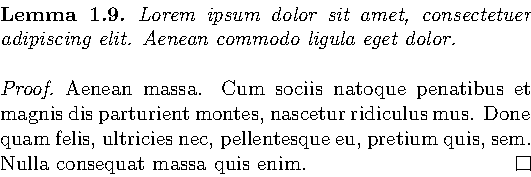
\includegraphics[width=\linewidth,height=0.8\textheight,keepaspectratio]{assets/latexRepeatEl.pdf}
            \end{column}
        \end{columns}
    \end{frame}

    \begin{frame}
        \frametitle{Code vs Visueel}

        \only<-1>{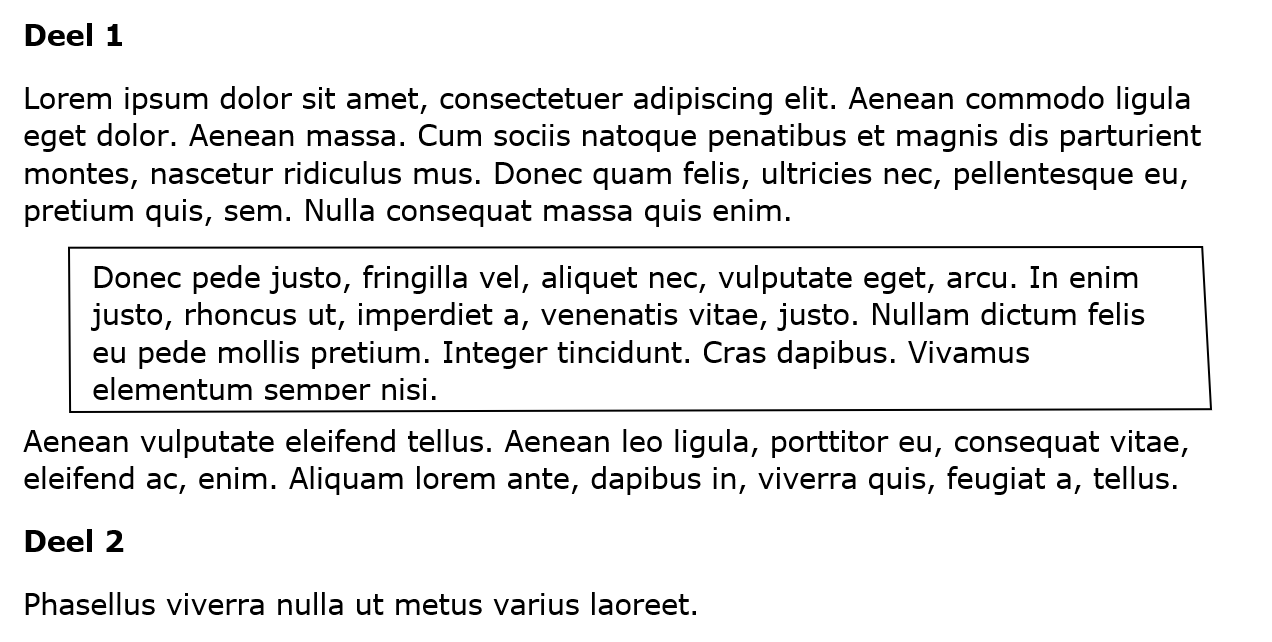
\includegraphics[width=\linewidth,height=0.8\textheight,keepaspectratio]{assets/wordkader2.png}}
        \unless\ifishandout
            \only<2->{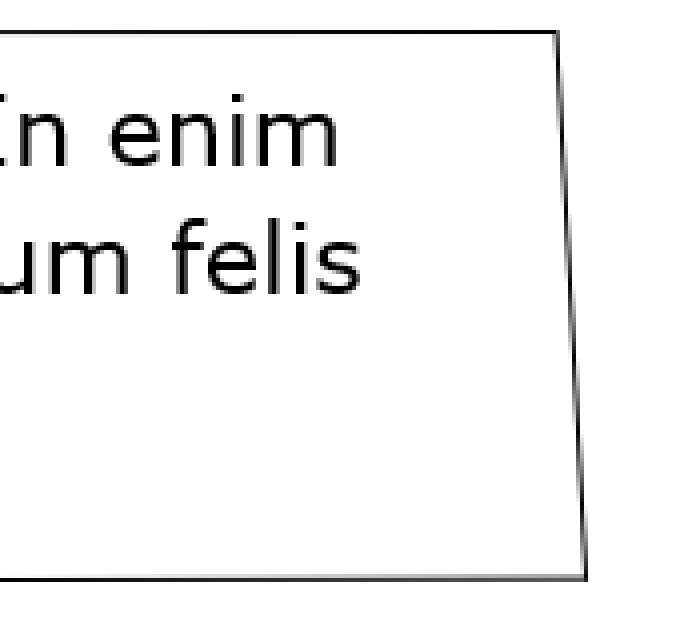
\includegraphics[width=\linewidth,height=0.8\textheight,keepaspectratio]{assets/wordkaderRand.png}}
        \fi

    \end{frame}

    \againframe<5->{codeoverview}

    \addtorecentlist{Overleaf}

    \begin{frame}
        \frametitle{Overleaf}

        %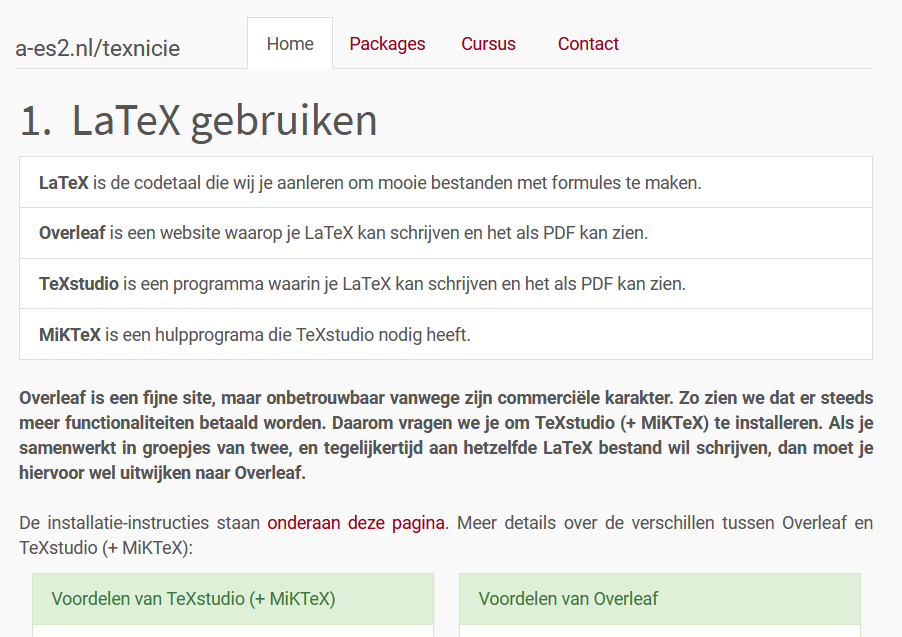
\includegraphics[trim=10px 120px 50px 30px,clip,width=0.95\textwidth]{texnicieWebsiteOverleafTeXstudio.png}
        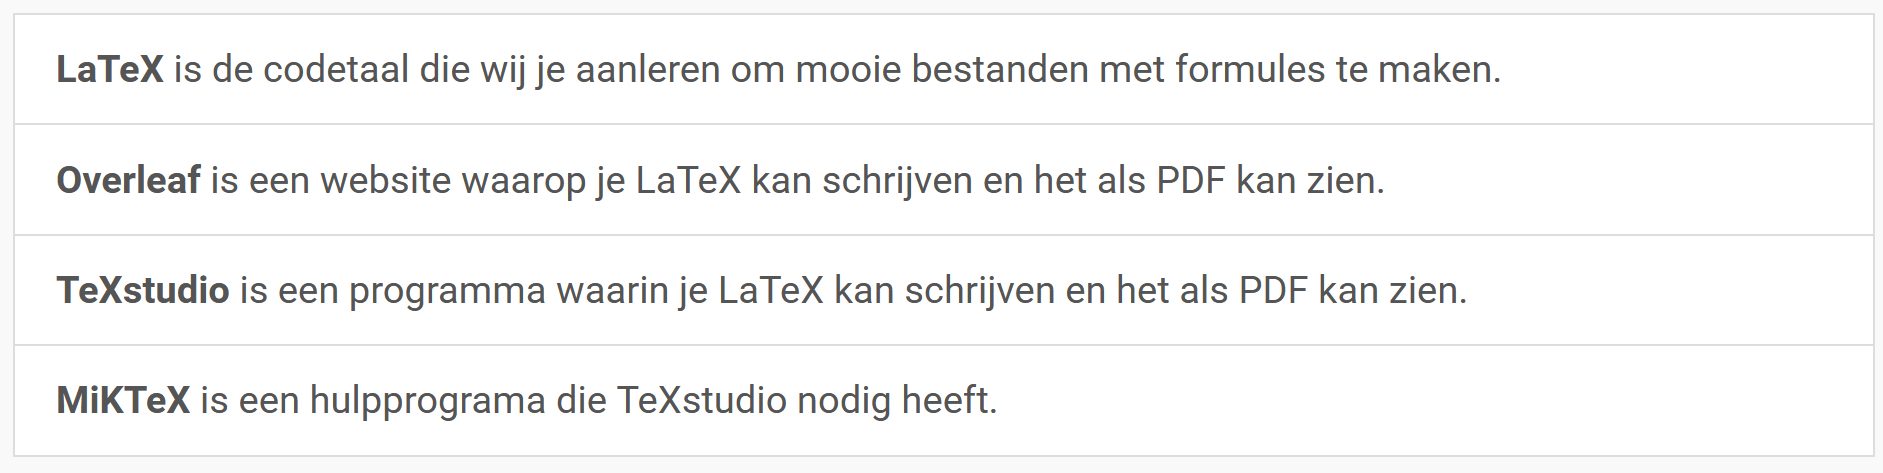
\includegraphics[width=\textwidth]{assets/overleafDisambiguation.png}

        \begin{columns}
            \begin{column}{0.3\textwidth}
                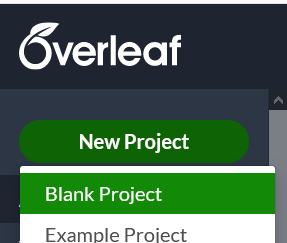
\includegraphics[width=\linewidth]{assets/overleafCreateBlankProject.png}
            \end{column}
            \begin{column}{0.7\textwidth}
                Op het einde nog woordje hierover.

                Voor nu: Overleaf.

                \medskip
                Nu al niet-commerci\"ele variant installeren? \url{a-es2.nl/texnicie}
            \end{column}
        \end{columns}
    \end{frame}

    \begin{saveblock}{baseDocument}
        \begin{highlightblock}[linewidth=0.5\textwidth,gobble=12]
            \documentclass{article}
            \usepackage[utf8]{inputenc}

            \title{My document}
            \author{Vincent Kuhlmann}
            \date{1 May 2021}

            \begin{document}
            \maketitle
            \section{Introduction}

            Hallo iedereen!
            \end{document}
        \end{highlightblock}
    \end{saveblock}

    \addtorecentlist{simpel document}

    \begin{frame}
        \frametitle{Simpel document}

        \begin{columns}
            \begin{column}{0.5\textwidth}
                \useblock{baseDocument}
            \end{column}
            \begin{column}{0.5\textwidth}
                
\includegraphics[width=\linewidth]{assets/basicDocumentOutput.png}
            \end{column}
        \end{columns}
    \end{frame}
\end{document}
\inputentrance
